\begin{figure*}[hbtp]
  \centering
  \subfigure[Runtime in seconds (logarithmic scale) for link prediction using various similarity measures, with \textit{LHub} approach]{
    \label{fig:pruned2--runtime}
    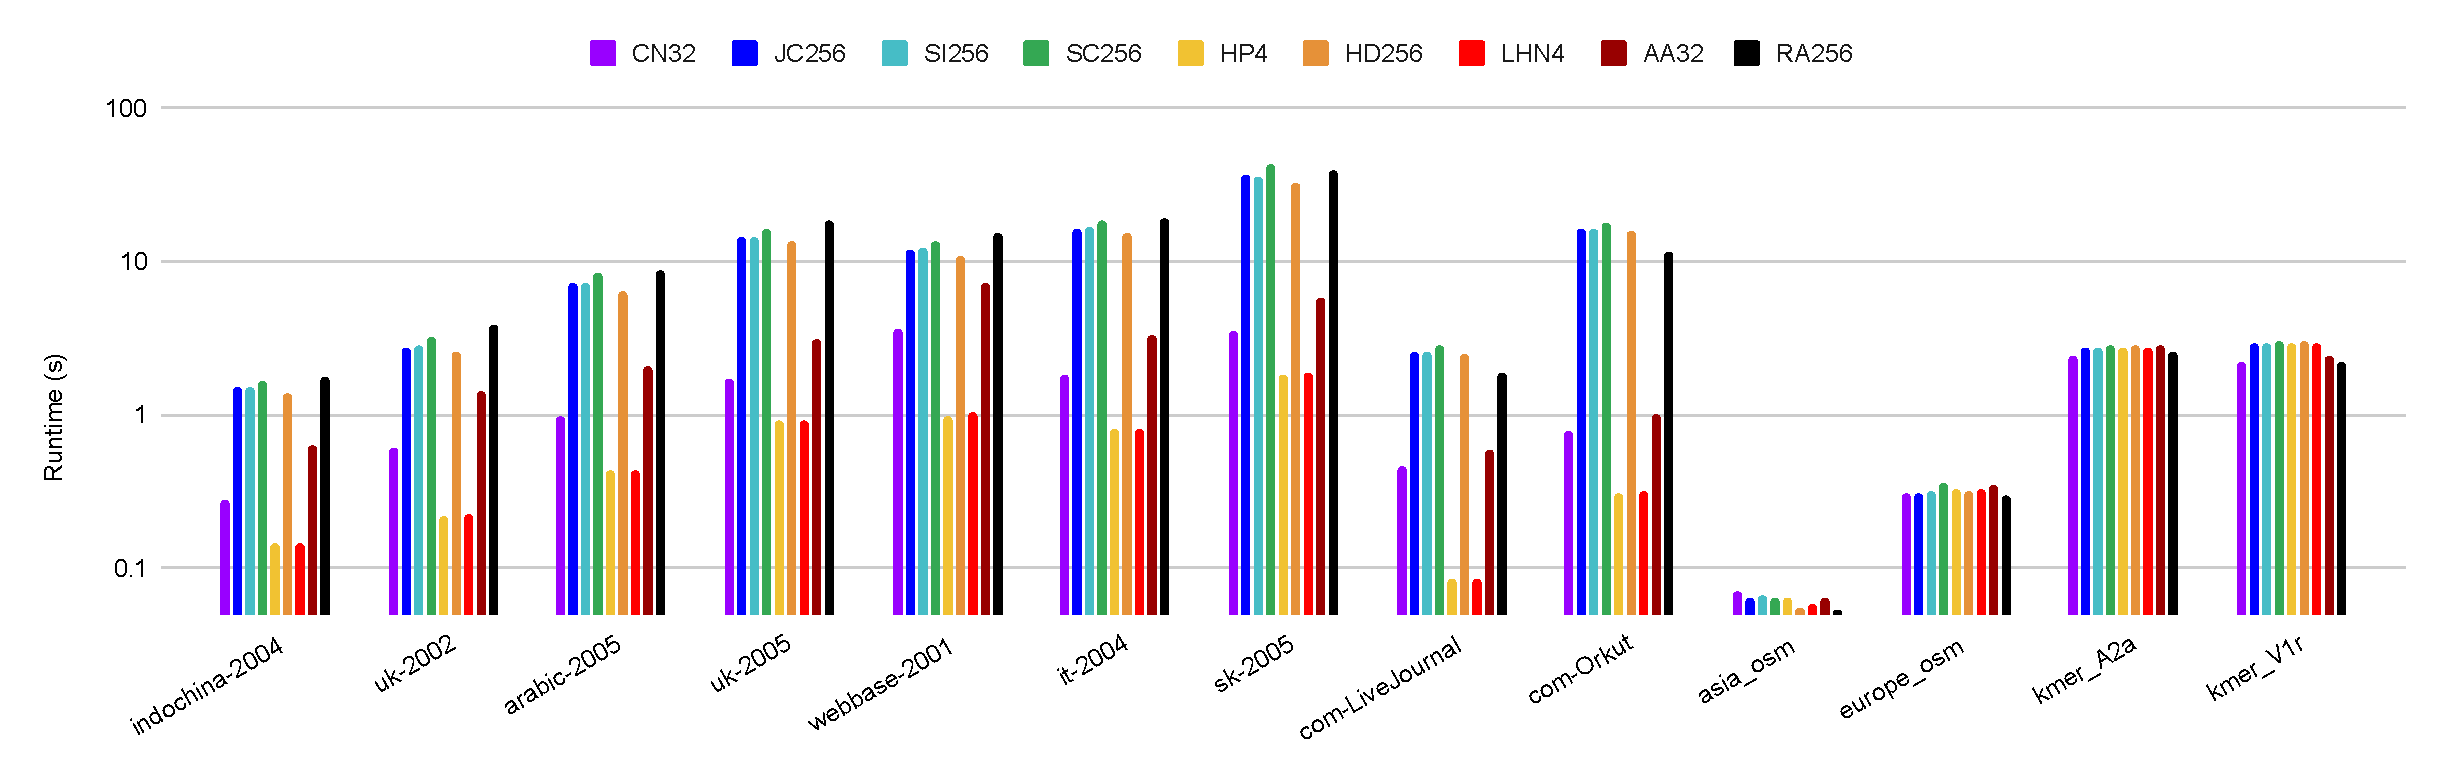
\includegraphics[width=0.98\linewidth]{out/pruned2-runtime.pdf}
  }
  \subfigure[F1 score of predicted links (logarithmic scale) for link prediction using various similarity measures, with \textit{LHub} approach]{
    \label{fig:pruned2--f1score}
    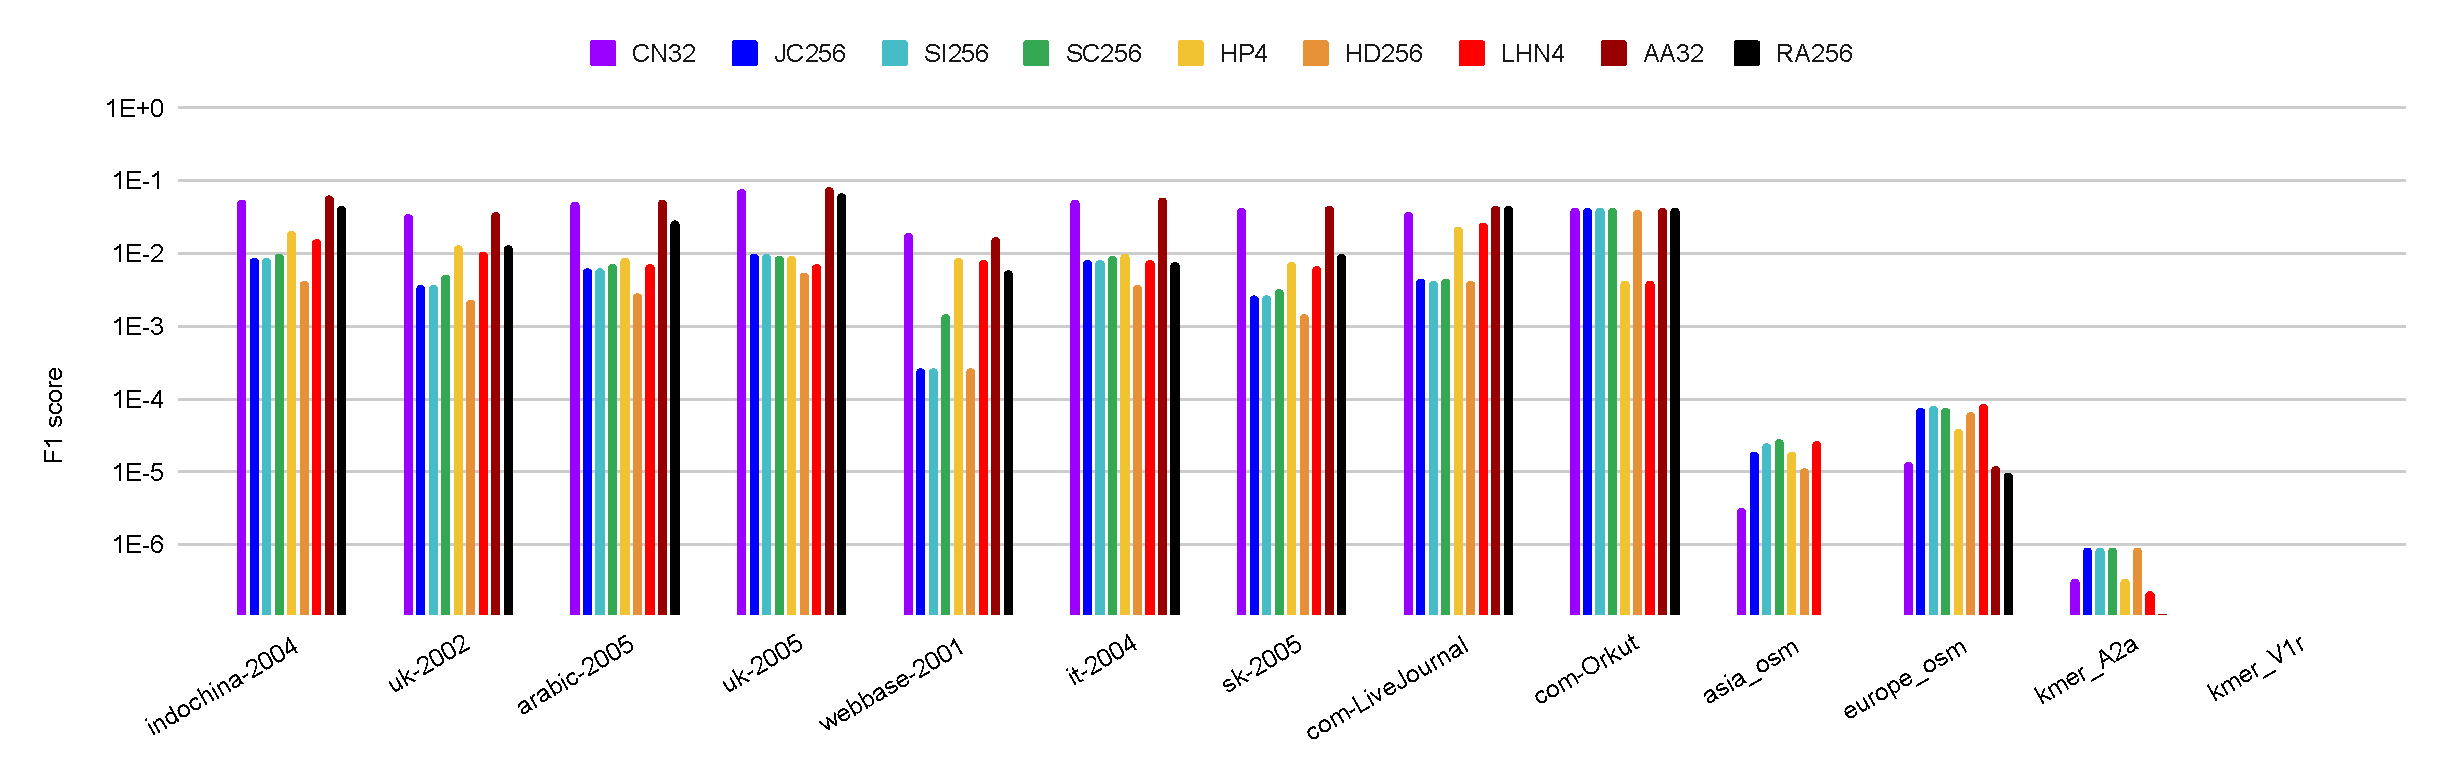
\includegraphics[width=0.98\linewidth]{out/pruned2-f1score.pdf}
  } \\[-2ex]
  \caption{Runtime (log-scale) and F1 score (log-scale) for link prediction using various similarity measures with the \textit{LHub} approach, when attempting to predict $10^{-2}|E|$ unobserved edges $E^U$ for each graph in the dataset. For each similarity measure outlined in Section \ref{sec:metrics}, the best hub limit $L_H$ parameter setting obtained in Section \ref{sec:select-limit} is used, indicated by a numerical suffix added to each link prediction method acronym.}
  \label{fig:pruned2}
\end{figure*}
